%%=========================================
\chapter{Results Not Included in the Main Report}\label{AppendixA}
This appendix displays all results that were not relevant enough to be a part of the results chapter. This mostly consists of the social networks from the later experiments. The results not included from experiments 6b and 7b will not be shown because they were conducted with one specific purpose, so the other graphs are not relevant.

\clearpage
\section{Experiment 4}

\begin{figure}[htbp]
    \subfigure[]{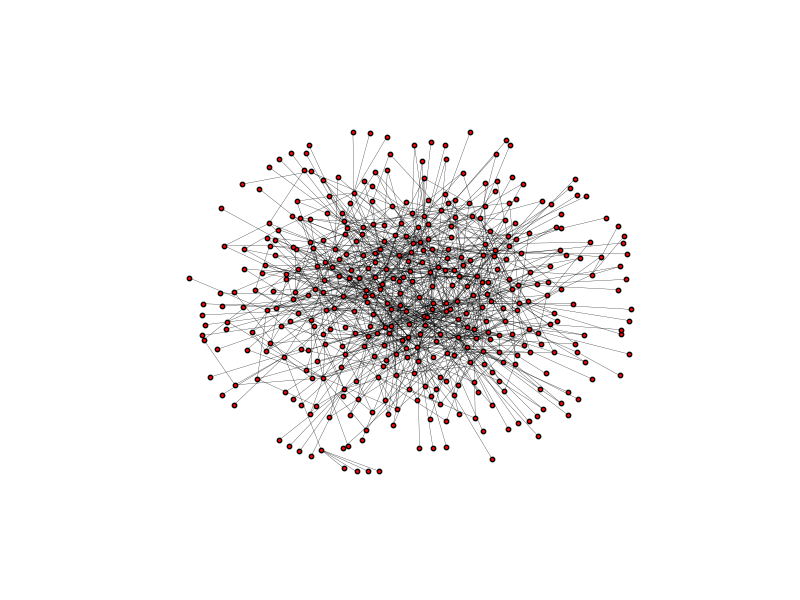
\includegraphics[width=0.49\linewidth]{fig/Results/Exp4/_graph5}\label{fig:exp4SN5}}
    \hfill
    \subfigure[]{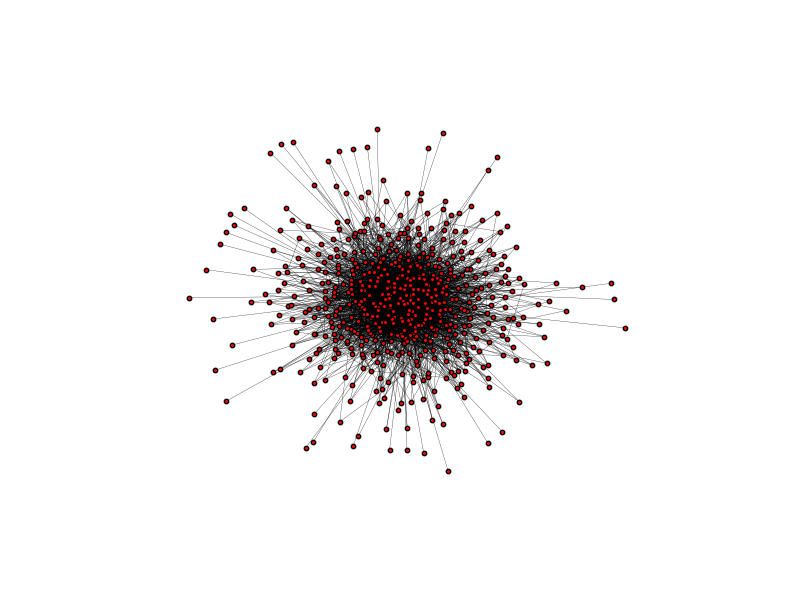
\includegraphics[width=0.49\linewidth]{fig/Results/Exp4/_graph20}\label{fig:exp4SN20}}
    \par \bigskip
    \subfigure[]{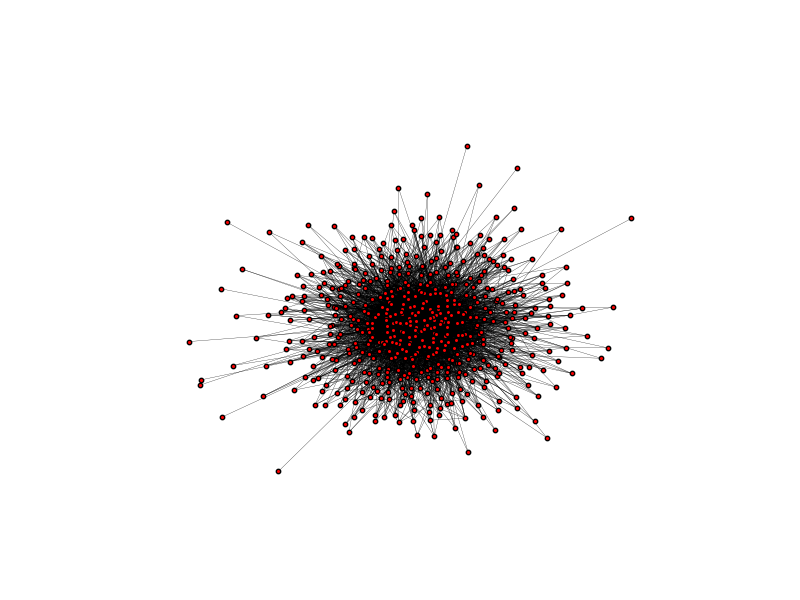
\includegraphics[width=0.49\linewidth]{fig/Results/Exp4/_graph40}\label{fig:exp4SN40}}
    \hfill
    \subfigure[]{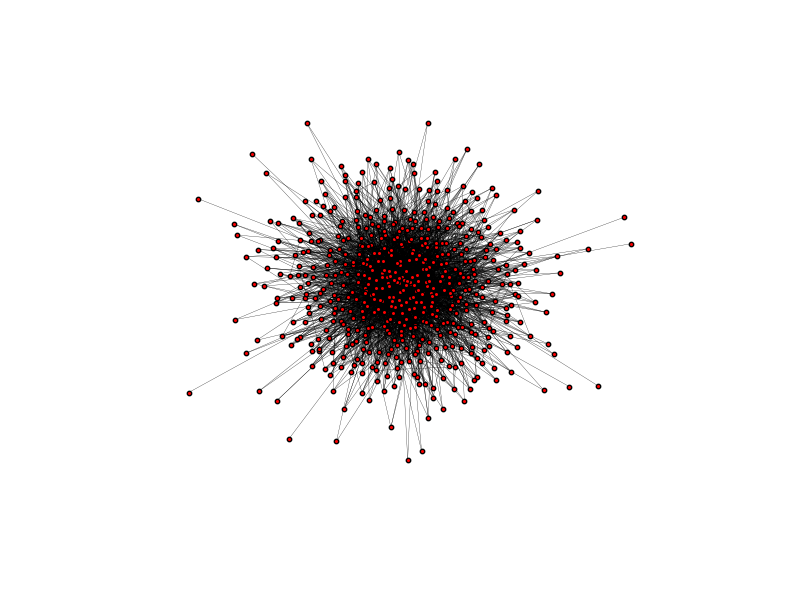
\includegraphics[width=0.49\linewidth]{fig/Results/Exp4/_graph100}\label{fig:exp4SN100}}
    \caption[Snapshots of the social network of experiment 4 at the following generations: 5, 20, 40, and 100.]{Snapshots of the social network of experiment 4 at the following generations: \subref{fig:exp4SN5} 5, \subref{fig:exp4SN20} 20, \subref{fig:exp4SN40} 40, and \subref{fig:exp4SN100} 100.}
    \label{fig:Appendix4}
\end{figure}

\clearpage
\section{Experiment 5}

\begin{figure}[htbp]
    \centering
    \subfigure[]{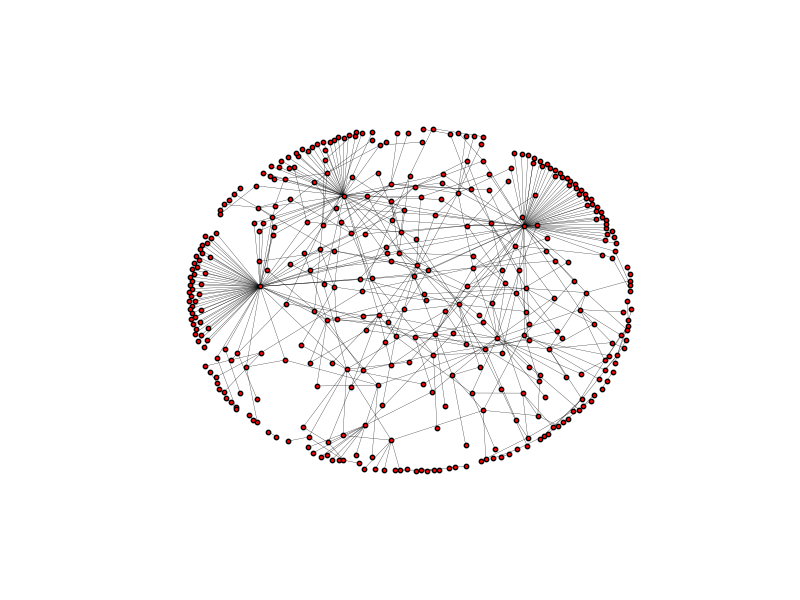
\includegraphics[width=0.49\linewidth]{fig/Results/Exp5/_graph5}\label{fig:exp5SN5}}
    \hfill
    \subfigure[]{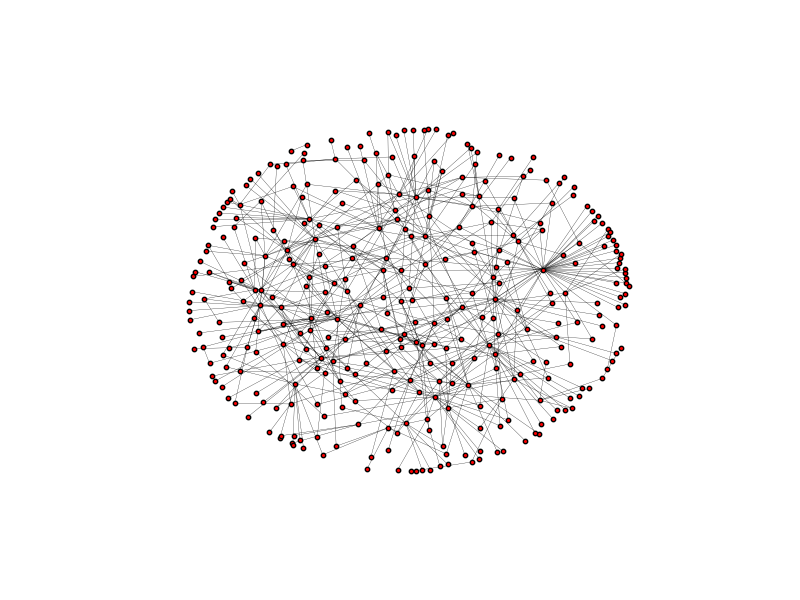
\includegraphics[width=0.49\linewidth]{fig/Results/Exp5/_graph20}\label{fig:exp5SN20}}
    \par \bigskip
    \subfigure[]{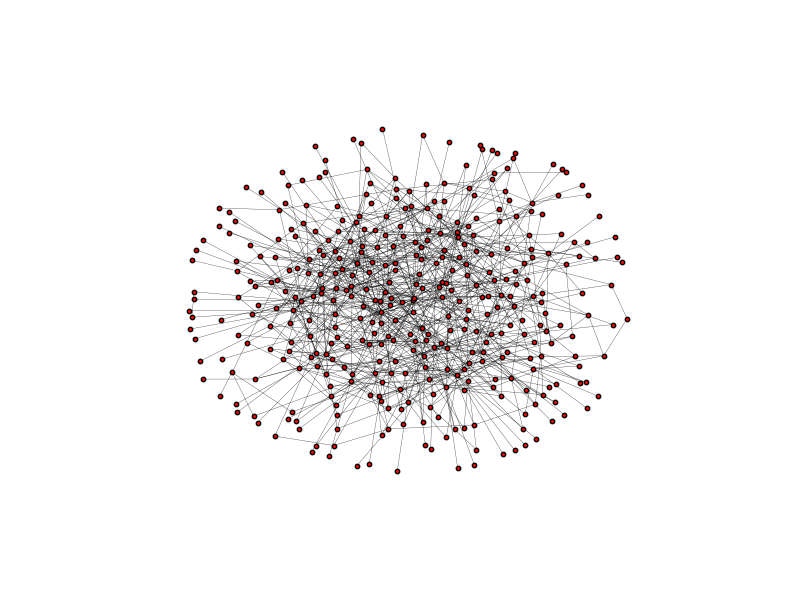
\includegraphics[width=0.49\linewidth]{fig/Results/Exp5/_graph100}\label{fig:exp5SN100}}
    \hfill
    \subfigure[]{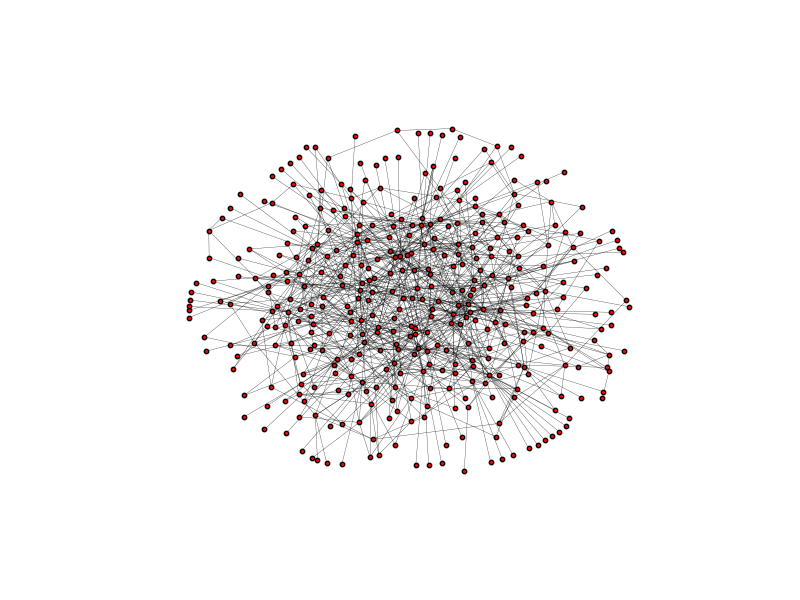
\includegraphics[width=0.49\linewidth]{fig/Results/Exp5/_graph150}\label{fig:exp5SN150}}
    \caption[Snapshots of the social network of experiment 5 at the following generations: 5, 20, 100, and 150.]{Snapshots of the social network of experiment 5 at the following generations: \subref{fig:exp5SN5} 5, \subref{fig:exp5SN20} 20, \subref{fig:exp5SN100} 100, and \subref{fig:exp5SN150} 150.}
\end{figure}

\clearpage
\section{Experiment 6}

\begin{figure}[htbp]
    \centering
    \subfigure[]{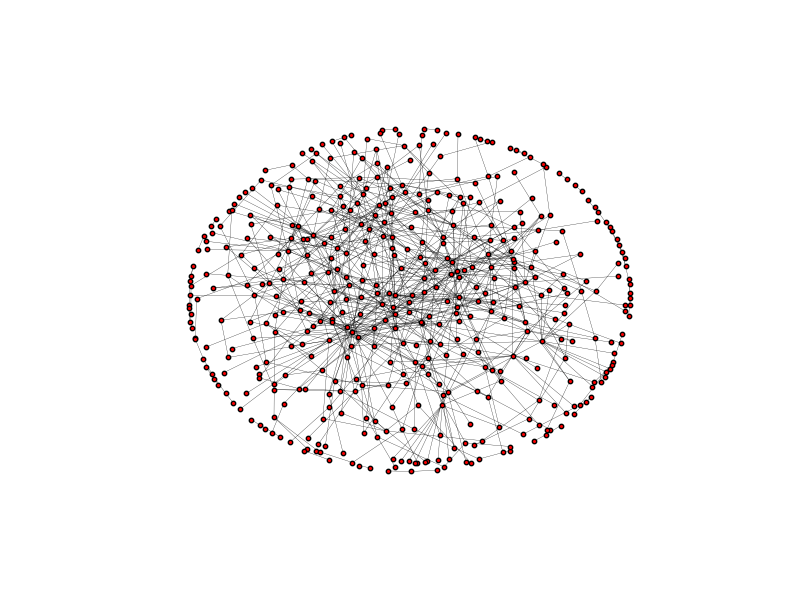
\includegraphics[width=0.49\linewidth]{fig/Results/Exp6/_graph5}\label{fig:exp6SN5}}
    \hfill
    \subfigure[]{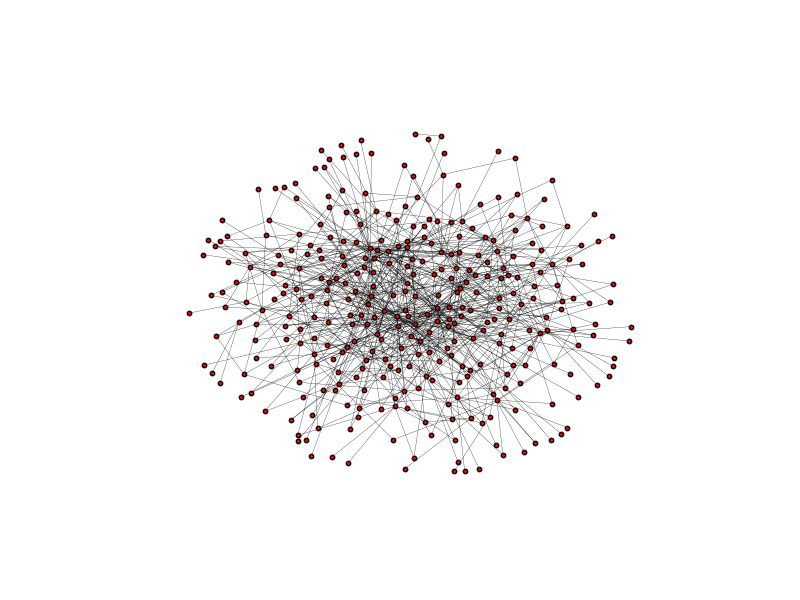
\includegraphics[width=0.49\linewidth]{fig/Results/Exp6/_graph20}\label{fig:exp6SN20}}
    \par \bigskip
    \subfigure[]{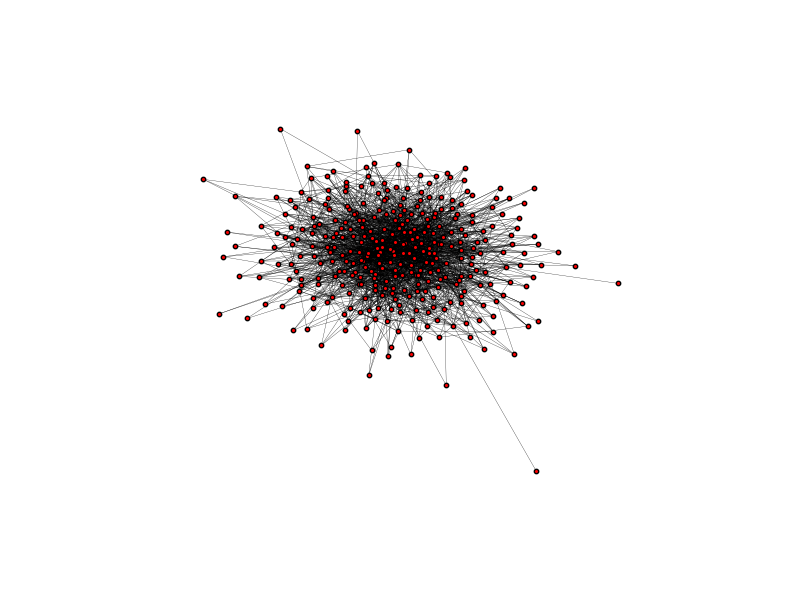
\includegraphics[width=0.49\linewidth]{fig/Results/Exp6/_graph100}\label{fig:exp6SN100}}
    \hfill
    \subfigure[]{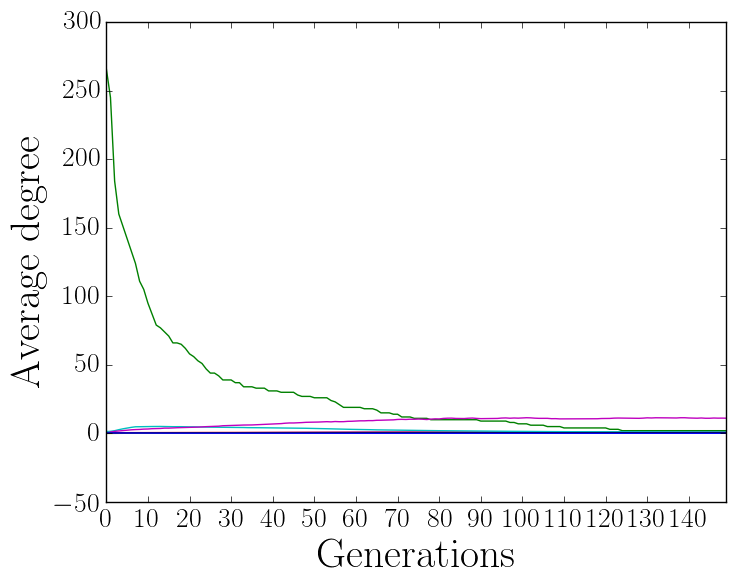
\includegraphics[width=0.49\linewidth]{fig/Results/Exp6/Genes1}\label{fig:Genes6}}
    \caption[Snapshots of the social network of experiment 6 at the following generations: 5, 20, and 100, and graphs showing the evolution of the the traits in the genome.]{Snapshots of the social network of experiment 6 at the following generations: \subref{fig:exp6SN5} 5, \subref{fig:exp6SN20} 20, and \subref{fig:exp6SN100} 100. \subref{fig:Genes6} Three graphs that show the evolution of the the traits in the genome. The green function represents the average probability of conducting parent-child dialogues, the blue function represents the average learning rate, and the red function represents the average probability of acting extrovertly.}
\end{figure}

\clearpage
\section{Experiment 7}
\begin{figure}[htbp]
    \centering
    \subfigure[]{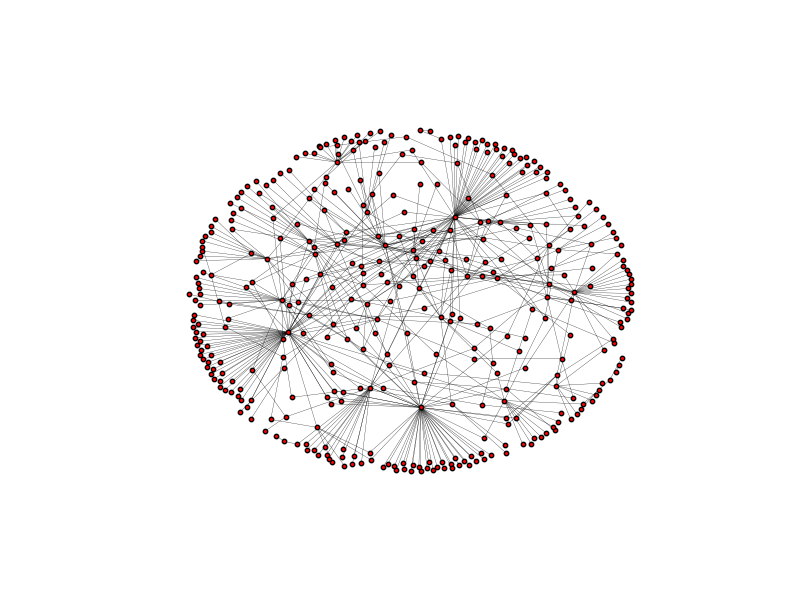
\includegraphics[width=0.49\linewidth]{fig/Results/Exp7/_graph5}\label{fig:exp7SN5}}
    \hfill
    \subfigure[]{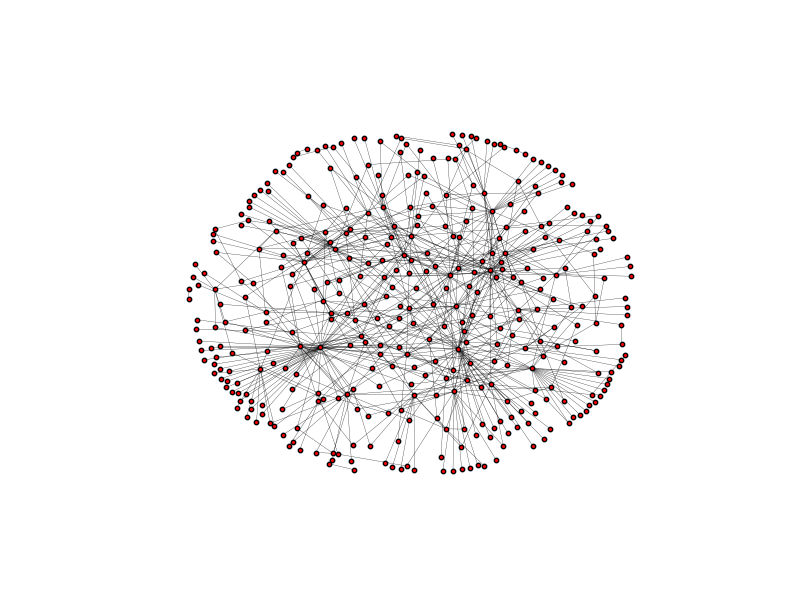
\includegraphics[width=0.49\linewidth]{fig/Results/Exp7/_graph20}\label{fig:exp7SN20}}
    \par \bigskip
    \subfigure[]{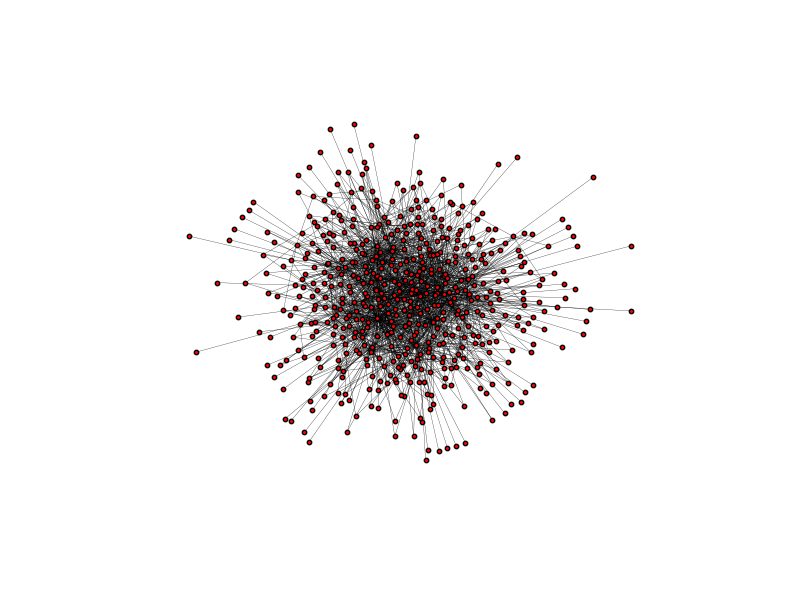
\includegraphics[width=0.49\linewidth]{fig/Results/Exp7/_graph100}\label{fig:exp7SN100}}
    \caption[Snapshots of the social network of experiment 7 at the following generations: 5, 20, and 100.]{Snapshots of the social network of experiment 7 at the following generations: \subref{fig:exp7SN5} 5, \subref{fig:exp7SN20} 20, and \subref{fig:exp7SN100} 100.}
\end{figure}
